%%%%%%%%%%%%%%%%%%%%%%%%%%%%%%%%%%%%%%%%%
% Masters/Doctoral Thesis 
% LaTeX Template
% Version 1.43 (17/5/14)
%
% This template has been downloaded from:
% http://www.LaTeXTemplates.com
%
% Original authors:
% Steven Gunn 
% http://users.ecs.soton.ac.uk/srg/softwaretools/document/templates/
% and
% Sunil Patel
% http://www.sunilpatel.co.uk/thesis-template/
%
% License:
% CC BY-NC-SA 3.0 (http://creativecommons.org/licenses/by-nc-sa/3.0/)
%
% Note:
% Make sure to edit document variables in the Thesis.cls file
%
%%%%%%%%%%%%%%%%%%%%%%%%%%%%%%%%%%%%%%%%%

%----------------------------------------------------------------------------------------
%	PACKAGES AND OTHER DOCUMENT CONFIGURATIONS
%----------------------------------------------------------------------------------------

\documentclass[11pt, oneside]{Thesis} % The default font size and one-sided printing (no margin offsets)

\graphicspath{{Pictures/}} % Specifies the directory where pictures are stored

\usepackage[square, numbers, comma, sort&compress]{natbib} % Use the natbib reference package - read up on this to edit the reference style; if you want text (e.g. Smith et al., 2012) for the in-text references (instead of numbers), remove 'numbers' 
\hypersetup{urlcolor=blue, colorlinks=true} % Colors hyperlinks in blue - change to black if annoying
\title{\ttitle} % Defines the thesis title - don't touch this

\begin{document}

\frontmatter % Use roman page numbering style (i, ii, iii, iv...) for the pre-content pages

\setstretch{1.3} % Line spacing of 1.3

% Define the page headers using the FancyHdr package and set up for one-sided printing
\fancyhead{} % Clears all page headers and footers
\rhead{\thepage} % Sets the right side header to show the page number
\lhead{} % Clears the left side page header

\pagestyle{fancy} % Finally, use the "fancy" page style to implement the FancyHdr headers

\newcommand{\HRule}{\rule{\linewidth}{0.5mm}} % New command to make the lines in the title page

% PDF meta-data
\hypersetup{pdftitle={\ttitle}}
\hypersetup{pdfsubject=\subjectname}
\hypersetup{pdfauthor=\authornames}
\hypersetup{pdfkeywords=\keywordnames}

%----------------------------------------------------------------------------------------
%	TITLE PAGE
%----------------------------------------------------------------------------------------

\begin{titlepage}
\begin{center}

\textsc{\LARGE \univname}\\[1.5cm] % University name
\textsc{\Large Project }\\[0.5cm] % Thesis type

\HRule \\[0.4cm] % Horizontal line
{\huge \bfseries \ttitle}\\[0.4cm] % Thesis title
\HRule \\[1.5cm] % Horizontal line
 
\begin{minipage}{0.4\textwidth}
\begin{flushleft} \large
\emph{Author:}\\
\href{http://www.johnsmith.com}{\authornames} % Author name - remove the \href bracket to remove the link
\end{flushleft}
\end{minipage}
\begin{minipage}{0.4\textwidth}
\begin{flushright} \large
\emph{Supervisor:} \\
\href{http://www.jamessmith.com}{\supname} % Supervisor name - remove the \href bracket to remove the link  
\end{flushright}
\end{minipage}\\[3cm]
 
%\large \textit{A thesis submitted in fulfilment of the requirements\\ for the degree of \degreename}\\[0.3cm] % University requirement text
%\textit{in the}\\[0.4cm]
\groupname\\\deptname\\[2cm] % Research group name and department name
 
{\large \today}\\[4cm] % Date
%\includegraphics{Logo} % University/department logo - uncomment to place it
 
\vfill
\end{center}

\end{titlepage}
%%fakesection - Declaration of Authorship
%----------------------------------------------------------------------------------------
%	DECLARATION PAGE
%	Your institution may give you a different text to place here
%----------------------------------------------------------------------------------------
%\Declaration{

%\addtocontents{toc}{\vspace{1em}} % Add a gap in the Contents, for aesthetics

%I, \authornames, declare that this thesis titled, '\ttitle' and the work presented in it are my own. I confirm that:

%\begin{itemize} 
%\item[\tiny{$\blacksquare$}] This work was done wholly or mainly while in candidature for a research degree at this University.
%\item[\tiny{$\blacksquare$}] Where any part of this thesis has previously been submitted for a degree or any other qualification at this University or any other institution, this has been clearly stated.
%\item[\tiny{$\blacksquare$}] Where I have consulted the published work of others, this is always clearly attributed.
%\item[\tiny{$\blacksquare$}] Where I have quoted from the work of others, the source is always given. With the exception of such quotations, this thesis is entirely my own work.
%\item[\tiny{$\blacksquare$}] I have acknowledged all main sources of help.
%\item[\tiny{$\blacksquare$}] Where the thesis is based on work done by myself jointly with others, I have made clear exactly what was done by others and what I have contributed myself.\\
%\end{itemize}
 
%Signed:\\
%\rule[1em]{25em}{0.5pt} % This prints a line for the signature
 
%Date:\\
%\rule[1em]{25em}{0.5pt} % This prints a line to write the date
%}

%\clearpage % Start a new page
%%fakesection - Quotation page
%----------------------------------------------------------------------------------------
%	QUOTATION PAGE
%----------------------------------------------------------------------------------------

%\pagestyle{empty} % No headers or footers for the following pages

%\null\vfill % Add some space to move the quote down the page a bit

%\textit{``Thanks to my solid academic training, today I can write hundreds of words on virtually any topic without possessing a shred of information, which is how I got a good job in journalism."}

%\begin{flushright}
%Dave Barry
%\end{flushright}

%\vfill\vfill\vfill\vfill\vfill\vfill\null % Add some space at the bottom to position the quote just right

%\clearpage % Start a new page

%----------------------------------------------------------------------------------------
%	ABSTRACT PAGE
%----------------------------------------------------------------------------------------
%%fakesection - Abstract
\addtotoc{Abstract} % Add the "Abstract" page entry to the Contents

\abstract{\addtocontents{toc}{\vspace{1em}} % Add a gap in the Contents, for aesthetics
In this project some basic properties of the least squares method is analysed. Both spectral and finite element basis functions are used in the implementation. The problem analysed in this projects are diffusion convection reaction problems, both linear and non-linear. The results are compared to standard Galerkin method. The least squares method is also applied as a smoothner with great results.  
}

\clearpage % Start a new page

%%fakesection - Acknowledgements 
%----------------------------------------------------------------------------------------
%	ACKNOWLEDGEMENTS
%----------------------------------------------------------------------------------------

%\setstretch{1.3} % Reset the line-spacing to 1.3 for body text (if it has changed)

%\acknowledgements{\addtocontents{toc}{\vspace{1em}} % Add a gap in the Contents, for aesthetics

%The acknowledgements and the people to thank go here, don't forget to include your project advisor\ldots
%}
%\clearpage % Start a new page

%%fakesection - List of contents/figs/tables
%----------------------------------------------------------------------------------------
%	LIST OF CONTENTS/FIGURES/TABLES PAGES
%----------------------------------------------------------------------------------------

\pagestyle{fancy} % The page style headers have been "empty" all this time, now use the "fancy" headers as defined before to bring them back

\lhead{\emph{Contents}} % Set the left side page header to "Contents"
\tableofcontents % Write out the Table of Contents

%\lhead{\emph{List of Figures}} % Set the left side page header to "List of Figures"
%\listoffigures % Write out the List of Figures

%\lhead{\emph{List of Tables}} % Set the left side page header to "List of Tables"
%\listoftables % Write out the List of Tables

%%fakesection - Abbreviations
%----------------------------------------------------------------------------------------
%	ABBREVIATIONS
%----------------------------------------------------------------------------------------

%\clearpage % Start a new page

%\setstretch{1.5} % Set the line spacing to 1.5, this makes the following tables easier to read

%\lhead{\emph{Abbreviations}} % Set the left side page header to "Abbreviations"
%\listofsymbols{ll} % Include a list of Abbreviations (a table of two columns)
%{
%\textbf{LAH} & \textbf{L}ist \textbf{A}bbreviations \textbf{H}ere \\
%%\textbf{Acronym} & \textbf{W}hat (it) \textbf{S}tands \textbf{F}or \\
%}

%%fakesection - Constants/Definitions 
%----------------------------------------------------------------------------------------
%	PHYSICAL CONSTANTS/OTHER DEFINITIONS
%----------------------------------------------------------------------------------------

%\clearpage % Start a new page

%\lhead{\emph{Physical Constants}} % Set the left side page header to "Physical Constants"

%\listofconstants{lrcl} % Include a list of Physical Constants (a four column table)
%{
%Speed of Light & $c$ & $=$ & $2.997\ 924\ 58\times10^{8}\ \mbox{ms}^{-\mbox{s}}$ (exact)\\
%% Constant Name & Symbol & = & Constant Value (with units) \\
%}

%%fakesection - Symbols 
%----------------------------------------------------------------------------------------
%	SYMBOLS
%----------------------------------------------------------------------------------------

%\clearpage % Start a new page

%\lhead{\emph{Symbols}} % Set the left side page header to "Symbols"

%\listofnomenclature{lll} % Include a list of Symbols (a three column table)
%{
%$a$ & distance & m \\
%$P$ & power & W (Js$^{-1}$) \\
%% Symbol & Name & Unit \\

%& & \\ % Gap to separate the Roman symbols from the Greek

%$\omega$ & angular frequency & rads$^{-1}$ \\
%% Symbol & Name & Unit \\
%}

%%fakesection - Dedication
%----------------------------------------------------------------------------------------
%	DEDICATION
%----------------------------------------------------------------------------------------

%\setstretch{1.3} % Return the line spacing back to 1.3

%\pagestyle{empty} % Page style needs to be empty for this page

%\dedicatory{For/Dedicated to/To my\ldots} % Dedication text

%\addtocontents{toc}{\vspace{2em}} % Add a gap in the Contents, for aesthetics

%----------------------------------------------------------------------------------------
%	THESIS CONTENT - CHAPTERS
%----------------------------------------------------------------------------------------

%%fakesection - Notation 
%----------------------------------------------------------------------------------------
%	NOTATION
%----------------------------------------------------------------------------------------

\clearpage % Start a new page

\setstretch{1.5} % Set the line spacing to 1.5, this makes the following tables easier to read

\lhead{\emph{Notation}} % Set the left side page header to "Abbreviations"
\listofsymbols{ll} % Include a list of Abbreviations (a table of two columns)
{
\textbf{CONVENTION} & we let subscript $h$ denote the discretized variables \\
$u$ & Solution of the partial differential equation\\
$\mathbf{w} = [w_1 \; w_2 ] $ & Negative gradient of $u$ \\
$\mathbf{u} = [ \mathbf{w} \; u ]^T$ & Solution to the first order transformation \\ 
$ R_g $ & Lifting function \\
$\tilde{\mathbf{u}} = \mathbf{u}-R_g $ & Solution to the first order transformation minus the lifting function \\ 
$\mathbf{b}$ & Two dimensional vector field \\
$f$ & loading function\\
$\mathbf{f} = (0,0,f)$ & loading function for the first order transformation\\
$\mathcal{L} , \mathcal{B} $ & Linear operators \\
$(\cdot,\cdot)$ & Inner product, when not specified read as $(\cdot,\cdot)_{L_2}$  \\
$a(\cdot,\cdot)$ & Bilinear form obtained from standard Galerkin approach \\
$Q(\cdot,\cdot)$ & Bilinear form obtained from the least squares approach \\
$\mathring{a}(\cdot,\cdot)$ & Bilinear form obtained from the combined GLS-method\\
$F(\cdot)$ & Linear form obtained from the least squares approach \\
$\tilde{F}(\cdot)$ & Linear form obtained from the least squares approach including BC's \\
$\mathring{F}(\cdot)$ & Linear form obtained from the combined GLS-method \\
\textbf{Linear Algebra} \\
$A$ & The stiffness matrix \\
$G$ & The gradient matrix \\
$R$ & The reaction matrix \\
$F$ & The vector obtained from the linear functional $F(\cdot)$ \\ 
$W$ 	& The diagonal matrix with the GLL-weights \\ 
$L$ 	& The matrix with the derivative of the lagrange functions evaluated in each node \\ 
%$\Phi$ & $W\otimes WL$\\ 
%$\Psi$ & $WL\otimes W$\\ 

%\textbf{LAH} & \textbf{L}ist \textbf{A}bbreviations \textbf{H}ere \\
%\textbf{Acronym} & \textbf{W}hat (it) \textbf{S}tands \textbf{F}or \\
}

\mainmatter % Begin numeric (1,2,3...) page numbering

\pagestyle{fancy} % Return the page headers back to the "fancy" style

% Include the chapters of the thesis as separate files from the Chapters folder
% Uncomment the lines as you write the chapters

%% Chapter 1

\chapter{Chapter Title Here} % Main chapter title

\label{Chapter1} % For referencing the chapter elsewhere, use \ref{Chapter1} 

\lhead{Chapter 1. \emph{Chapter Title Here}} % This is for the header on each page - perhaps a shortened title

%----------------------------------------------------------------------------------------

\section{Welcome and Thank You}
Welcome to this \LaTeX{} Thesis Template, a beautiful and easy to use template for writing a thesis using the \LaTeX{} typesetting system.

If you are writing a thesis (or will be in the future) and its subject is technical or mathematical (though it doesn't have to be), then creating it in \LaTeX{} is highly recommended as a way to make sure you can just get down to the essential writing without having to worry over formatting or wasting time arguing with your word processor.

\LaTeX{} is easily able to professionally typeset documents that run to hundreds or thousands of pages long. With simple mark-up commands, it automatically sets out the table of contents, margins, page headers and footers and keeps the formatting consistent and beautiful. One of its main strengths is the way it can easily typeset mathematics, even \emph{heavy} mathematics. Even if those equations are the most horribly twisted and most difficult mathematical problems that can only be solved on a super-computer, you can at least count on \LaTeX{} to make them look stunning.

%----------------------------------------------------------------------------------------

\section{Learning \LaTeX{}}

\LaTeX{} is not a WYSIWYG (What You See is What You Get) program, unlike word processors such as Microsoft Word or Apple's Pages. Instead, a document written for \LaTeX{} is actually a simple, plain text file that contains \emph{no formatting}. You tell \LaTeX{} how you want the formatting in the finished document by writing in simple commands amongst the text, for example, if I want to use \textit{italic text for emphasis}, I write the `$\backslash$\texttt{textit}\{\}' command and put the text I want in italics in between the curly braces. This means that \LaTeX{} is a ``mark-up'' language, very much like HTML.

\subsection{A (not so short) Introduction to \LaTeX{}}

If you are new to \LaTeX{}, there is a very good eBook -- freely available online as a PDF file -- called, ``The Not So Short Introduction to \LaTeX{}''. The book's title is typically shortened to just ``lshort''. You can download the latest version (as it is occasionally updated) from here:\\
\href{http://www.ctan.org/tex-archive/info/lshort/english/lshort.pdf}{\texttt{http://www.ctan.org/tex-archive/info/lshort/english/lshort.pdf}}

It is also available in several other languages. Find yours from the list on this page:\\
\href{http://www.ctan.org/tex-archive/info/lshort/}{\texttt{http://www.ctan.org/tex-archive/info/lshort/}}

It is recommended to take a little time out to learn how to use \LaTeX{} by creating several, small `test' documents. Making the effort now means you're not stuck learning the system when what you \emph{really} need to be doing is writing your thesis.

\subsection{A Short Math Guide for \LaTeX{}}

If you are writing a technical or mathematical thesis, then you may want to read the document by the AMS (American Mathematical Society) called, ``A Short Math Guide for \LaTeX{}''. It can be found online here:\\
\href{http://www.ams.org/tex/amslatex.html}{\texttt{http://www.ams.org/tex/amslatex.html}}\\
under the ``Additional Documentation'' section towards the bottom of the page.

\subsection{Common \LaTeX{} Math Symbols}
There are a multitude of mathematical symbols available for \LaTeX{} and it would take a great effort to learn the commands for them all. The most common ones you are likely to use are shown on this page:\\
\href{http://www.sunilpatel.co.uk/latexsymbols.html}{\texttt{http://www.sunilpatel.co.uk/latexsymbols.html}}

You can use this page as a reference or crib sheet, the symbols are rendered as large, high quality images so you can quickly find the \LaTeX{} command for the symbol you need.

\subsection{\LaTeX{} on a Mac}
 
The \LaTeX{} package is available for many systems including Windows, Linux and Mac OS X. The package for OS X is called MacTeX and it contains all the applications you need -- bundled together and pre-customised -- for a fully working \LaTeX{} environment and workflow.
 
MacTeX includes a dedicated \LaTeX{} IDE (Integrated Development Environment) called ``TeXShop'' for writing your `\texttt{.tex}' files and ``BibDesk'': a program to manage your references and create your bibliography section just as easily as managing songs and creating playlists in iTunes.

%----------------------------------------------------------------------------------------

\section{Getting Started with this Template}

If you are familiar with \LaTeX{}, then you can familiarise yourself with the contents of the Zip file and the directory structure and then place your own information into the `\texttt{Thesis.cls}' file. Section \ref{FillingFile} on page \pageref{FillingFile} tells you how to do this. Make sure you read section \ref{ThesisConventions} about thesis conventions to get the most out of this template and then get started with the `\texttt{Thesis.tex}' file straightaway.

If you are new to \LaTeX{} it is recommended that you carry on reading through the rest of the information in this document.

\subsection{About this Template}

This \LaTeX{} Thesis Template is originally based and created around a \LaTeX{} style file created by Steve R.\ Gunn from the University of Southampton (UK), department of Electronics and Computer Science. You can find his original thesis style file at his site, here:\\
\href{http://www.ecs.soton.ac.uk/~srg/softwaretools/document/templates/}{\texttt{http://www.ecs.soton.ac.uk/$\sim$srg/softwaretools/document/templates/}}

My thesis originally used the `\texttt{ecsthesis.cls}' from his list of styles. However, I knew \LaTeX{} could still format better. To get the look I wanted, I modified his style and also created a skeleton framework and folder structure to place the thesis files in.

This Thesis Template consists of that modified style, the framework and the folder structure. All the work that has gone into the preparation and groundwork means that all you have to bother about is the writing.

Before you begin using this template you should ensure that its style complies with the thesis style guidelines imposed by your institution. In most cases this template style and layout will be suitable. If it is not, it may only require a small change to bring the template in line with your institution's recommendations.

%----------------------------------------------------------------------------------------

\section{What this Template Includes}

\subsection{Folders}

This template comes as a single Zip file that expands out to many files and folders. The folder names are mostly self-explanatory:

\textbf{Appendices} -- this is the folder where you put the appendices. Each appendix should go into its own separate `\texttt{.tex}' file. A template is included in the directory.

\textbf{Chapters} -- this is the folder where you put the thesis chapters. A thesis usually has about seven chapters, though there is no hard rule on this. Each chapter should go in its own separate `\texttt{.tex}' file and they usually are split as:
\begin{itemize}
\item Chapter 1: Introduction to the thesis topic
\item Chapter 2: Background information and theory
\item Chapter 3: (Laboratory) experimental setup
\item Chapter 4: Details of experiment 1
\item Chapter 5: Details of experiment 2
\item Chapter 6: Discussion of the experimental results
\item Chapter 7: Conclusion and future directions
\end{itemize}
This chapter layout is specialised for the experimental sciences.

\textbf{Figures} -- this folder contains all figures for the thesis. These are the final images that will go into the thesis document.

\textbf{Primitives} -- this is the folder that contains scraps, particularly because one final image in the `Figures' folder may be made from many separate images and photos, these source images go here. This keeps the intermediate files separate from the final thesis figures.

\subsection{Files}

Included are also several files, most of them are plain text and you can see their contents in a text editor. Luckily, many of them are auxiliary files created by \LaTeX{} or BibTeX and which you don't need to bother about:

\textbf{Bibliography.bib} -- this is an important file that contains all the bibliographic information and references that you will be citing in the thesis for use with BibTeX. You can write it manually, but there are reference manager programs available that will create and manage it for you. Bibliographies in \LaTeX{} are a large subject and you may need to read about BibTeX before starting with this.

\textbf{Thesis.cls} -- this is an important file. It is the style file that tells \LaTeX{} how to format the thesis. You will also need to open this file in a text editor and fill in your own information (such as name, department, institution). Luckily, this is not too difficult and is explained in section \ref{FillingFile} on page \pageref{FillingFile}.

\textbf{Thesis.pdf} -- this is your beautifully typeset thesis (in the PDF file format) created by \LaTeX{}.

\textbf{Thesis.tex} -- this is an important file. This is the file that you tell \LaTeX{} to compile to produce your thesis as a PDF file. It contains the framework and constructs that tell \LaTeX{} how to layout the thesis. It is heavily commented so you can read exactly what each line of code does and why it is there. After you put your own information into the `\texttt{Thesis.cls}' file, go to this file and begin filling it in -- you have now started your thesis!

\textbf{vector.sty} -- this is a \LaTeX{} package, it tells \LaTeX{} how to typeset mathematical vectors. Using this package is very easy and you can read the documentation on the site (you just need to look at the `\texttt{vector.pdf}' file):\\
\href{http://www.ctan.org/tex-archive/macros/latex/contrib/vector/}{\texttt{http://www.ctan.org/tex-archive/macros/latex/contrib/vector/}}

\textbf{lstpatch.sty} -- this is a \LaTeX{} package required by this LaTeX template and is included as not all \TeX{} distributions have it installed by default. You do not need to modify this file.

Files that are \emph{not} included, but are created by \LaTeX{} as auxiliary files include:

\textbf{Thesis.aux} -- this is an auxiliary file generated by \LaTeX{}, if it is deleted \LaTeX{} simply regenerates it when you run the main `\texttt{.tex}' file.

\textbf{Thesis.bbl} -- this is an auxiliary file generated by BibTeX, if it is deleted, BibTeX simply regenerates it when you run the main tex file. Whereas the `\texttt{.bib}' file contains all the references you have, this `\texttt{.bbl}' file contains the references you have actually cited in the thesis and is used to build the bibliography section of the thesis.

\textbf{Thesis.blg} -- this is an auxiliary file generated by BibTeX, if it is deleted BibTeX simply regenerates it when you run the main `\texttt{.tex}' file.

\textbf{Thesis.lof} -- this is an auxiliary file generated by \LaTeX{}, if it is deleted \LaTeX{} simply regenerates it when you run the main `\texttt{.tex}' file. It tells \LaTeX{} how to build the `List of Figures' section.

\textbf{Thesis.log} -- this is an auxiliary file generated by \LaTeX{}, if it is deleted \LaTeX{} simply regenerates it when you run the main `\texttt{.tex}' file. It contains messages from \LaTeX{}, if you receive errors and warnings from \LaTeX{}, they will be in this `\texttt{.log}' file.

\textbf{Thesis.lot} -- this is an auxiliary file generated by \LaTeX{}, if it is deleted \LaTeX{} simply regenerates it when you run the main `\texttt{.tex}' file. It tells \LaTeX{} how to build the `List of Tables' section.

\textbf{Thesis.out} -- this is an auxiliary file generated by \LaTeX{}, if it is deleted \LaTeX{} simply regenerates it when you run the main `\texttt{.tex}' file.


So from this long list, only the files with the `\texttt{.sty}', `\texttt{.bib}', `\texttt{.cls}' and `\texttt{.tex}' extensions are the most important ones. The other auxiliary files can be ignored or deleted as \LaTeX{} and BibTeX will regenerate them.

%----------------------------------------------------------------------------------------

\section{Filling in the `\texttt{Thesis.cls}' File}\label{FillingFile}

You will need to personalise the thesis template and make it your own by filling in your own information. This is done by editing the `\texttt{Thesis.cls}' file in a text editor.

Open the file and scroll down, past all the `$\backslash$\texttt{newcommand}\ldots' items until you see the entries for `\texttt{University Name}', `\texttt{Department Name}', etc\ldots.

Fill out the information about your group and institution and ensure you keep to block capitals where it asks you to. You can also insert web links, if you do, make sure you use the full URL, including the `\texttt{http://}' for this.

The last item you should need to fill in is the Faculty Name (in block capitals). When you have done this, save the file and recompile `\texttt{Thesis.tex}'. All the information you filled in should now be in the PDF, complete with web links. You can now begin your thesis proper!

%----------------------------------------------------------------------------------------

\section{The `\texttt{Thesis.tex}' File Explained}

The \texttt{Thesis.tex} file contains the structure of the thesis. There are plenty of written comments that explain what pages, sections and formatting the \LaTeX{} code is creating. Initially there seems to be a lot of \LaTeX{} code, but this is all formatting, and it has all been taken care of so you don't have to do it.

Begin by checking that your information on the title page is correct. For the thesis declaration, your institution may insist on something different than the text given. If this is the case, just replace what you see with what is required.

Then comes a page which contains a funny quote. You can put your own, or quote your favourite scientist, author, person, etc\ldots Make sure to put the name of the person who you took the quote from.

Next comes the acknowledgements. On this page, write about all the people who you wish to thank (not forgetting parents, partners and your advisor/supervisor).

The contents pages, list of figures and tables are all taken care of for you and do not need to be manually created or edited. The next set of pages are optional and can be deleted since they are for a more technical thesis: insert a list of abbreviations you have used in the thesis, then a list of the physical constants and numbers you refer to and finally, a list of mathematical symbols used in any formulae. Making the effort to fill these tables means the reader has a one-stop place to refer to instead of searching the internet and references to try and find out what you meant by certain abbreviations or symbols.

The list of symbols is split into the Roman and Greek alphabets. Whereas the abbreviations and symbols ought to be listed in alphabetical order (and this is \emph{not} done automatically for you) the list of physical constants should be grouped into similar themes.

The next page contains a one line dedication. Who will you dedicate your thesis to?

Finally, there is the section where the chapters are included. Uncomment the lines (delete the `\texttt{\%}' character) as you write the chapters. Each chapter should be written in its own file and put into the `Chapters' folder and named `\texttt{Chapter1}', `\texttt{Chapter2}, etc\ldots Similarly for the appendices, uncomment the lines as you need them. Each appendix should go into its own file and placed in the `Appendices' folder.

After the preamble, chapters and appendices finally comes the bibliography. The bibliography style (called `\texttt{unsrtnat}') is used for the bibliography and is a fully featured style that will even include links to where the referenced paper can be found online. Do not under estimate how grateful you reader will be to find that a reference to a paper is just a click away. Of course, this relies on you putting the URL information into the BibTeX file in the first place.

%----------------------------------------------------------------------------------------

\section{Thesis Features and Conventions}\label{ThesisConventions}

To get the best out of this template, there are a few conventions that you may want to follow.

One of the most important (and most difficult) things to keep track of in such a long document as a thesis is consistency. Using certain conventions and ways of doing things (such as using a Todo list) makes the job easier. Of course, all of these are optional and you can adopt your own method.

\subsection{Printing Format}

This thesis template is designed for single sided printing as most theses are printed and bound this way. This means that the left margin is always wider than the right (for binding). Four out of five people will now judge the margins by eye and think, ``I never 
noticed that before.''.

The headers for the pages contain the page number on the right side (so it is easy to flick through to the page you want) and the chapter name on the left side.

The text is set to 11 point and a line spacing of 1.3. Generally, it is much more readable to have a smaller text size and wider gap between the lines than it is to have a larger text size and smaller gap. Again, you can tune the text size and spacing should you want or need to. The text size can be set in the options for the `$\backslash$\texttt{documentclass}' command at the top of the `\texttt{Thesis.tex}' file and the spacing can be changed by setting a different value in the `$\backslash$\texttt{setstretch}' commands (scattered throughout the `\texttt{Thesis.tex}' file).

\subsection{Using US Letter Paper}

The paper size used in the template is A4, which is a common -- if not standard -- size in Europe. If you are using this thesis template elsewhere and particularly in the United States, then you may have to change the A4 paper size to the US Letter size. Unfortunately, this is not as simple as replacing instances of `\texttt{a4paper}' with `\texttt{letterpaper}'.

This is because the final PDF file is created directly from the \LaTeX{} source using a program called `\texttt{pdfTeX}' and in certain conditions, paper size commands are ignored and all documents are created with the paper size set to the size stated in the configuration file for pdfTeX (called `\texttt{pdftex.cfg}').

What needs to be done is to change the paper size in the configuration file for \texttt{pdfTeX} to reflect the letter size. There is an excellent tutorial on how to do this here: \\
\href{http://www.physics.wm.edu/~norman/latexhints/pdf_papersize.html}{\texttt{http://www.physics.wm.edu/$\sim$norman/latexhints/pdf\_papersize.html}}

It may be sufficient just to replace the dimensions of the A4 paper size with the US Letter size in the \texttt{pdftex.cfg} file. Due to the differences in the paper size, the resulting margins may be different to what you like or require (as it is common for Institutions to dictate certain margin sizes). If this is the case, then the margin sizes can be tweaked by opening up the \texttt{Thesis.cls} file and searching for the line beginning with, `$\backslash$\texttt{setmarginsrb}' (not very far down from the top), there you will see the margins specified. Simply change those values to what you need (or what looks good) and save. Now your document should be set up for US Letter paper size with suitable margins.

\subsection{References}

The `\texttt{natbib}' package is used to format the bibliography and inserts references such as this one \citep{Reference3}. The options used in the `\texttt{Thesis.tex}' file mean that the references are listed in numerical order as they appear in the text. Multiple references are rearranged in numerical order (e.g. \citep{Reference2, Reference1}) and multiple, sequential references become reformatted to a reference range (e.g. \citep{Reference2, Reference1, Reference3}). This is done automatically for you. To see how you use references, have a look at the `\texttt{Chapter1.tex}' source file. Many reference managers allow you to simply drag the reference into the document as you type.

Scientific references should come \emph{before} the punctuation mark if there is one (such as a comma or period). The same goes for footnotes\footnote{Such as this footnote, here down at the bottom of the page.}. You can change this but the most important thing is to keep the convention consistent throughout the thesis. Footnotes themselves should be full, descriptive sentences (beginning with a capital letter and ending with a full stop).

To see how \LaTeX{} typesets the bibliography, have a look at the very end of this document (or just click on the reference number links).

\subsection{Figures}

There will hopefully be many figures in your thesis (that should be placed in the `Figures' folder). The way to insert figures into your thesis is to use a code template like this:
\begin{verbatim}
\begin{figure}[htbp]
  \centering
    
\includegraphics{Figures/Electron.pdf}
    \rule{35em}{0.5pt}
  \caption[An Electron]{An electron (artist's impression).}
  \label{fig:Electron}
\end{figure}
\end{verbatim}
Also look in the source file. Putting this code into the source file produces the picture of the electron that you can see in the figure below.

\begin{figure}[htbp]
	\centering
		
\includegraphics{Figures/Electron.pdf}
		\rule{35em}{0.5pt}
	\caption[An Electron]{An electron (artist's impression).}
	\label{fig:Electron}
\end{figure}

Sometimes figures don't always appear where you write them in the source. The placement depends on how much space there is on the page for the figure. Sometimes there is not enough room to fit a figure directly where it should go (in relation to the text) and so \LaTeX{} puts it at the top of the next page. Positioning figures is the job of \LaTeX{} and so you should only worry about making them look good!

Figures usually should have labels just in case you need to refer to them (such as in Figure \ref{fig:Electron}). The `$\backslash$\texttt{caption}' command contains two parts, the first part, inside the square brackets is the title that will appear in the `List of Figures', and so should be short. The second part in the curly brackets should contain the longer and more descriptive caption text.

The `$\backslash$\texttt{rule}' command is optional and simply puts an aesthetic horizontal line below the image. If you do this for one image, do it for all of them.

The \LaTeX{} Thesis Template is able to use figures that are either in the PDF or JPEG file format.

\subsection{Typesetting mathematics}

If your thesis is going to contain heavy mathematical content, be sure that \LaTeX{} will make it look beautiful, even though it won't be able to solve the equations for you.

The ``Not So Short Introduction to \LaTeX{}'' (available \href{http://www.ctan.org/tex-archive/info/lshort/english/lshort.pdf}{here}) should tell you everything you need to know for most cases of typesetting mathematics. If you need more information, a much more thorough mathematical guide is available from the AMS called, ``A Short Math Guide to \LaTeX{}'' and can be downloaded from:\\
\href{ftp://ftp.ams.org/pub/tex/doc/amsmath/short-math-guide.pdf}{\texttt{ftp://ftp.ams.org/pub/tex/doc/amsmath/short-math-guide.pdf}}

There are many different \LaTeX{} symbols to remember, luckily you can find the most common symbols \href{http://www.sunilpatel.co.uk/latexsymbols.html}{here}. You can use the web page as a quick reference or crib sheet and because the symbols are grouped and rendered as high quality images (each with a downloadable PDF), finding the symbol you need is quick and easy.

You can write an equation, which is automatically given an equation number by \LaTeX{} like this:
\begin{verbatim}
\begin{equation}
E = mc^{2}
  \label{eqn:Einstein}
\end{equation}
\end{verbatim}

This will produce Einstein's famous energy-matter equivalence equation:
\begin{equation}
E = mc^{2}
\label{eqn:Einstein}
\end{equation}

All equations you write (which are not in the middle of paragraph text) are automatically given equation numbers by \LaTeX{}. If you don't want a particular equation numbered, just put the command, `$\backslash$\texttt{nonumber}' immediately after the equation.

%----------------------------------------------------------------------------------------

\section{Sectioning and Subsectioning}

You should break your thesis up into nice, bite-sized sections and subsections. \LaTeX{} automatically builds a table of Contents by looking at all the `$\backslash$\texttt{chapter}$\{\}$', `$\backslash$\texttt{section}$\{\}$' and `$\backslash$\texttt{subsection}$\{\}$' commands you write in the source.

The table of Contents should only list the sections to three (3) levels. A `$\backslash$\texttt{chapter}$\{\}$' is level one (1). A `$\backslash$\texttt{section}$\{\}$' is level two (2) and so a `$\backslash$\texttt{subsection}$\{\}$' is level three (3). In your thesis it is likely that you will even use a `$\backslash$\texttt{subsubsection}$\{\}$', which is level four (4). Adding all these will create an unnecessarily cluttered table of Contents and so you should use the `$\backslash$\texttt{subsubsection$^{*}\{\}$}' command instead (note the asterisk). The asterisk ($^{*}$) tells \LaTeX{} to omit listing the subsubsection in the Contents, keeping it clean and tidy.

%----------------------------------------------------------------------------------------

\section{In Closing}

You have reached the end of this mini-guide. You can now rename or overwrite this pdf file and begin writing your own `\texttt{Chapter1.tex}' and the rest of your thesis. The easy work of setting up the structure and framework has been taken care of for you. It's now your job to fill it out!

Good luck and have lots of fun!

\begin{flushright}
Guide written by ---\\
Sunil Patel: \href{http://www.sunilpatel.co.uk}{www.sunilpatel.co.uk}
\end{flushright}

% Chapter 1 - THEORY

\chapter{Theory} % Main chapter title

\label{chap:theory} % For referencing the chapter elsewhere, use \ref{Chapter1} 

\lhead{Chapter 1. \emph{Established theory}} % This is for the header on each page - perhaps a shortened title

%----------------------------------------------------------------------------------------

\section{Informal introduction to least-squares}
The least-squares finite element method is a numerical method with similarities to mixed Galerkin. However it has a fundamentally different approach regarding the definition of the bilinear functional. Let us look at a system of first order differential equations on the form 
\begin{align}
	Au &= f \text{ in } \Omega \\
	u &= g \text{ on } \partial \Omega.
	\label{eq:PDE}
\end{align}
Where $A$ is a partial differential operator defined as 
\begin{align}
	A = \sum_{i = 1}^{n} A_i\frac{\partial}{\partial x_i} + A_0.
	\label{def:operatorA}
\end{align}
	$n$ being the number of dimensions of the domain $\Omega$. If $u$ happens to be a vector function of say $k$ dimensions then $A_i$ will be a matrix with $k$ columns and $k$ or more rows. Let us initially assume without loss of generality that $g=0$ . Further we require $f \in L_2(\Omega)$ and choose $V = \left\{ v\in L_2(\Omega) | v = 0 \text{ on } \partial \Omega \right\}$. A residual is defined
\begin{align}
	R(v) = Av-f,
	\label{eq:Residual}
\end{align}
and a functional
\begin{align}
	 J(v) = \frac{1}{2}||R(v)||^2_0.
	\label{eq:Functional}
\end{align} 
The solution $u$ and it's gradient needs to be in $L^2$ for the functional to make sense, hence $u$ is restricted to the space $H^1_0(\Omega)$. The homogeneous boundary condition is now baked into the definition of the search space. By minimizing $J$ we obtain 
\begin{align}
	\lim_{t\rightarrow 0} \frac{d}{dt}J(u+tv) = \int_{\Omega}(Av)^T(Au-f)d\Omega = 0 \text{    ,   } \forall v \in V.
	\label{eq:minProb}
\end{align}
We can now write a variational formulation of the least-squares method: Find $u \in V$ such that 
\begin{align}
	Q(u,v) = F(v) \; \; \; , \; \; \; \forall v \in V,
	\label{def:varForm}
\end{align}
where
\begin{align}
	Q(u,v) = (Au,Av), \\
	F(v) = (f,Av).
	\label{def:bilin}
\end{align}
Notice that the bilinear form $Q$ is symmetric, this is an important advantage least-squares has over regular Galerkin methods. The bilinear form that surged from a first-order problem by the least-squares leads us to a variational formulation similar to the one obtained from a second order problem by regular FEM. Generally the bilinear form from least-squares will correspond to a bilinear form of a problem of twice the order obtained using FEM. \colorbox{yellow}{Bold statement?} In order to avoid problems of large complexity a higher order PDE should therefore be transformed to a system of first order PDE's (similar to a mixed Galerkin approach) before defining the least squares functional.
\cite{Jiang}
%In order to apply a numerical algorithm the domain $\Omega$ needs to be discretized, we name this discretization $\Omega_h$. A set of basis functions $ \left\{ N \right\}_i $ is defined for $V_h = H^1_0(\Omega_h)$ such that the discrete variational formulation can be stated. Find $u_h \in V_h$ such that 
%\begin{align}
	%Q(u_h,v_h) = F(v_h) \; \; \; , \; \; \; \forall v_h \in V_h,
	%\label{def:varForm}
%\end{align}

\section{ Formal formulation of least-squares}
Let us look at a general boundary value problem where $f \in Y(\Omega)$, $g \in B(\partial \Omega)$, $\mathcal{B}\colon X(\partial \Omega) \to B(\partial\Omega) $ and $\mathcal{L}\colon X(\Omega)\to Y(\Omega)$. Find $u \in X(\Omega) $ such that 
\begin{align}
	\mathcal{L} u &= f \; \; \; \text{ in } \Omega \\
	\mathcal{B}u &= g \; \; \; \text{ on } \partial \Omega.
	\label{eq:BVP}
\end{align}
Whenever this BVP has a unique solution, a least-squares functional can be defined as 
\begin{align}
	J(u;f,g) = ||\mathcal{L}u-f||^2_Y + ||\mathcal{B}u-g||^2_B
	\label{eq:FunctionalGen}
\end{align}
and the corresponding minimization problem is then given as 
\begin{align}
	\min_{u \in X}J(u;f,g)
	\label{eq:minProbGen}
\end{align}
For any well-posed problem $\exists \alpha,\beta > 0$ such that 
\begin{align}
	\alpha||u||_X^2 \leq J(u;0,0) = (\mathcal{L}u,\mathcal{L}u)_Y+(\mathcal{B}u,\mathcal{B}u)_B \leq \beta||u||_X^2.
	\label{eq:normEq}
\end{align}
The fact that our functional is norm-equivalent is of crucial importance to a successful LS-method. It is therefore important that the spaces $X,Y \text{ and } B$ is chosen such that the LS-functional defines a norm is equivalent to $|| \cdot ||_X$.\colorbox{yellow}{Need to show this ? }
Minimizing this functional is equivalent to solving the Euler-Lagrange equations formulated as 
\begin{align}
	\text{find } u \in X \text{  such that  } Q(u,v) = F(v) \; \; \forall v\in X
	\label{eq:varFormGen}
\end{align}
Where $Q(u,v)$ and $F(v)$ are defined as 
\begin{align}
	Q(u,v) &= (\mathcal{L}u,\mathcal{L}v)_Y+(\mathcal{B}u,\mathcal{B}v)_B, \\
	F(v) &= (f,\mathcal{L}v)_Y+(g,\mathcal{L}v)_B.
	\label{VarFormLinForms}
\end{align}
%
Notice that $Q(u,v)$ defines an inner product and $Q(u,u)^{1/2}=J(u;0,0)^{1/2}$ defines the corresponding norm. 

In order to solve this numerically we define the function spaces $X^h, Y^h \text{ and } B^h$ and the corresponding variational formulation is then written as 
\begin{align}
	\text{find } u^h \in X^h \text{  such that  } Q(u^h,v^h) = F(v^h) \; \; \forall v^h\in X^h.
	\label{eq:varFormGenDisc}
\end{align}
~\cite{Bochev}
%
\subsection{Error analysis}
Let $u$ be the analytical solution of a problem of the type ~\eref{eq:BVP}, $u^h$ is our numerical solution to ~\eref{eq:varFormGenDisc} and $u^h_{\perp} $ is the orthogonal projection of $u$ in $X_h$. 
\begin{align}
	Q(u-u^h,u-u^h) &= Q(u-u^h,u-u^h_{\perp}) + Q(u-u^h,u^h_{\perp}-u^h) \\
							   &= Q(u-u^h,u-u^h_{\perp}) \\
							 	 &\leq \beta ||u-u^h||_{X_h} \; ||u-u^h_{\perp}||_{X_h}.
	\label{eq:error1}
\end{align}
The first equality is due to adding and subtracting $u^h_{\perp}$, because both $u^h$ and $u^h_{\perp}$ solves the variational formulation we can cancel the last term, and by using the norm-equivalency from ~\eref{eq:normEq} and Schwartz inequality we get the last  expression. Now by applying the first inequality of ~\eref{eq:normEq} we end up with 
\begin{align}
	||u-u^h||_{X_h}\leq \frac{\beta}{\alpha}||u-u^h_{\perp}||_{X_h} = \min_{w^h \in X_h}\frac{\beta}{\alpha}||u-w^h||_{X_h}.
	\label{error_final}
\end{align}
Hence we can show that the Least squares method provides a convergence result of similar order as the Finite element method.
\colorbox{yellow}{Add the convergence result of spectral methods}


\section{Example - Poisson problem}

The Poisson problem is defined as 
\begin{align}
	-\Delta u = f \text{ in } \Omega \\
	u = g \text{ on } \partial \Omega
	\label{eq:Poisson}
\end{align}
Let us first consider the homogeneous case. The straight forward least-squares approach is to define $\mathbf{w} = -\nabla u$ and solve the system of equations 
\begin{align}
	\mathbf{w} + \nabla u = 0 \text{ in } \Omega \\
	\nabla \cdot \mathbf{w} = f \text{ in } \Omega \\
	u = 0 \text{ on } \partial \Omega.
	\label{eq:PoissonSystem}
\end{align}
which can be written in the same form as ~\eref{eq:BVP} with $ \mathbf{u} = \mathbf{w} \oplus u $, $\mathbf{f} = (0,0,f)$, $g=0$, $\mathcal{B} = (0,0,1)^T $ and $\mathcal{L}$ given as 
\begin{align}
	\mathcal{L} =
	\begin{bmatrix}
		1 & 0 & \frac{\partial} {\partial x}  \\
		0 & 1 & \frac{\partial} {\partial y}  \\
    \frac{\partial} {\partial x} & \frac{\partial} {\partial y} & 0 
	\end{bmatrix}
	\label{eq:Amatrix}
\end{align}
We define the search space $X =  H^1(\Omega;\text{div}) \times H_0^1(\Omega)$ and the solution space $Y \times B  = [L^2(\Omega)]^3\times L^2(\Omega) $ and the functional can then be defined as in~\eref{eq:FunctionalGen}. The variational formulation of the problem can be stated. Find $ \mathbf{u} \in X $ such that
\begin{align}
	Q(\mathbf{u},\mathbf{v}) = F(\mathbf{v}) \;\; \forall \;\; \mathbf{v} \in X.
	\label{eq:VariationalFormulationPoisson}
\end{align}
We require that $\mathbf{f} \in Y$.
\colorbox{yellow}{Should I state the numerical variational formulation instead??}
Notice that the spaces $X$ and $Y$ chosen as described above fulfill the condition ~\eref{eq:normEq}. 
%
\section{Example - Diffusion transport reaction problem}
%
The diffusion transport reaction problem to be analyzed is given as 
\begin{align}
	-\mu \Delta u + \mathbf{b} \cdot \nabla u +\sigma u = f \text{ in } \Omega \\
	u = g \text{ on } \partial \Omega
	\label{eq:DiffTrans}
\end{align}
where $ \mu$ is the diffusion constant, $\mathbf{b} = [b_1 , b_2]$ is a vector field nd $\sigma$ is some reaction constant. By following the same approach as for the Poisson problem we end up with $\mathcal{L}$ on the form
\begin{align}
	\mathcal{L} =
	\begin{bmatrix}
		1 & 0 & \frac{\partial} {\partial x}  \\
		0 & 1 & \frac{\partial} {\partial y}  \\
		\mu \frac{\partial} {\partial x} - b_1 & \mu \frac{\partial} {\partial y} -b_2 & \sigma
	\end{bmatrix}
	\label{eq:AmatrixDiff}
\end{align}
which leads to a similar but slightly different linear system than the one created by the Poisson problem.

%The straight forward least-squares approach is to define $\mathbf{w} = -\nabla u$ and solve the system of equations \begin{align}
	%\mathbf{w} + \nabla u = 0 \text{ in } \Omega \\
	%\nabla \cdot \mathbf{w} - b \cdot \mathbf{w} = f \text{ in } \Omega \\
	%u = 0 \text{ on } \partial \Omega.
	%\label{eq:DiffTransSystem}
%\end{align}
%which can be written in the same form as ~\eref{eq:BVP} with $ \mathbf{u} = \mathbf{w} \oplus u $, $\mathbf{f} = (0,0,f)$, g = 0, $\mathcal{B} = (0,0,1)^T $ and L given as 
%\begin{align}
	%\mathcal{L} =
	%\begin{bmatrix}
		%1 & 0 & \partial / \partial x  \\
		%0 & 1 & \partial / \partial y  \\
		%\partial / \partial x - b_1 & \partial/ \partial y -b_2 & 0
	%\end{bmatrix}
	%\label{eq:AmatrixDiff}
%\end{align}
%We define the search space $X =  H^1(\Omega;\text{div}) \times H_0^1(\Omega)$ and the solution space $Y \times B  = [L^2(\Omega)]^3\times L^2(\Omega) $ and the functional can then be defined as in~\eref{eq:FunctionalGen}. The variational formulation of the problem can be stated. Find $ \mathbf{u} \in X $ s.t.
%\begin{align}
	%Q(\mathbf{u},\mathbf{v}) = F(\mathbf{v}) \;\; \forall \;\; \mathbf{v} \in X.
	%\label{eq:VariationalFormulationPoisson}
%\end{align}
%We require that $\mathbf{f} \in Y$.
%Notice that the spaces $X$ and $Y$ chosen as described above fullfill the condition ~\eref{eq:normEq}. 

\section{Boundary conditions}
\subsection{non-homogeneous Dirichlet boundary conditions}
If $g \neq 0$ then we simply define a lifting function $R_g \in X$ such that $R_g(\partial \Omega) = g(\partial \Omega)$. By defining $\tilde{\mathbf{u}}=\mathbf{u}-R_g$ we can replace $\mathbf{u}$ in the variation formulation and get 
\begin{align}
	Q(\tilde{\mathbf{u}}+R_g,\mathbf{v}) &= F(\mathbf{v}) \\
	Q(\tilde{\mathbf{u}},\mathbf{v})+Q(R_g,\mathbf{v}) &= F(\mathbf{v}) \\
	Q(\tilde{\mathbf{u}},\mathbf{v}) &= F(\mathbf{v}) - Q(R_g,\mathbf{v})\\
	Q(\tilde{\mathbf{u}},\mathbf{v}) &= \tilde{F}(\mathbf{v}) 
	\label{eq:liftingFunc}
\end{align}
%
\subsection{non-homogeneous Neumann boundary conditions}
Because of the geometry of our problem and the fact that we define the flux as an extra variable we can transform the Neumann conditions to a Dirichlet condition on the flux. 
\begin{align}
	\frac{\partial u}{\partial \mathbf{n}} &= h \text{  on   } \partial \Omega \\
	\nabla u \cdot \mathbf{n} &= h \\
	 \mathbf{w} \cdot \mathbf{n} &= -h. 
	\label{eq:neumann}
\end{align}
Let us define $\hat{x}$ and $\hat{y}$ as the unit vectors in each direction. Notice that for the west ($x=0$) and east ($x=1$) edges the normal vector $\mathbf{n}= \pm\hat{x}$, and at the north ($y=1$) and south($y=0$) edges $\mathbf{n}=\pm \hat{y}$. This way we can write the Neumann conditions as a Dirichlet condition on the first and second component of $\mathbf{w}= [ w_1 \:\: w_2]$. 
\begin{align}
	w_1 = \pm h \text{    for $y = 0$ and $y=1$ }\\
	w_2 = \pm h \text{    for $x = 0$ and $x=1$ }
	\label{eq:neumannAsDirichlet}
\end{align}
\subsection{Boundary as an additional functional}
The boundary conditions can also be implemented as the functional described in equation \eref{eq:FunctionalGen}. For a BVP with Dirichlet BC's this will correspon to adding $||u-g||^2_0$ to our functional $J$. By minimizing this term we end up with the following contribution to the variational form
\begin{align}
	(u,v)_{\partial \Omega}=(g,v)_{\partial \Omega}
	\label{eq:BCFunctionalImplementationContribution}
\end{align}
 
% Chapter 2 - NEW THEORY

\chapter{Stability properties of least-squares} % Main chapter title

\label{chap:newTheory} % For referencing the chapter elsewhere, use \ref{Chapter1} 

\lhead{Chapter 2. \emph{Stability properties }} % This is for the header on each page - perhaps a shortened title

%----------------------------------------------------------------------------------------
\section{Instability with the Galerkin formulation}

With regular Galerkin approach for the diffusion transport equation you end up with the variational formulation 
%
\begin{align}
	a(u,v) = (f,v) \; \; \; \forall v \in V.
	\label{eq:varFormDiffFEM}
\end{align}
%
where $V$ is some closed subspace of $H^1$, and the bilinear functional is given as 
%
\begin{align}
	\begin{split}
	a(u,v) &= \mu\int_{\Omega}\nabla u \cdot \nabla v \: d\Omega 
	+ \int_{\Omega} v (b \cdot \nabla u) d \Omega
	\end{split}
	\label{eq:bilinearFunctional}
\end{align}
%
We can define a new norm from this functional in the following manner
%
\begin{align}
\begin{split}
	a(u,u) &= \mu\int_{\Omega}\nabla u \cdot \nabla u \: d\Omega 
	+ \int_{\Omega}  b \cdot (u\nabla u) d \Omega\\
	       &= \mu||\nabla u||^2_0 
	+ \frac{1}{2}\int_{\Omega} b \cdot \nabla u^2 d \Omega \\
	       &= \mu||\nabla u||^2_0 
	- \frac{1}{2}\int_{\Omega} u^2  (\nabla \cdot b)  d \Omega \\
\end{split}
	\label{eq:bilinearFunctional}
\end{align}
%
Where we have used Greens theorem and the assumption that $u=0$ on the boundary in the last equality. Let us assume that the divergence of our vector field can be bounded within some interval, say  $\gamma_0 \leq -\frac{1}{2}\nabla \cdot b \leq \gamma_1 $, we can now make a lower and upper bound for the norm surging from the bilinear form 
%
\begin{align}
	\mu||\nabla u||^2_0 + \gamma_0||u||^2_0 \leq a(u,u) \leq \mu||\nabla u||^2_0 + \gamma_1||u||^2_0
	\label{eq:bilinearOperatorBounds}
\end{align}
%
It is clear that for negative $\gamma_0$ and sufficiently small $\mu$ the bilinear form is no longer coercive and thus our convergence requirements are no longer valid. Standard Galerkin method is therefore not a suited way to solve this type of problem. 
\section{Adding least squares in order to obtain stability}

Now remember from equation \eref{eq:normEq} that the least squares formulation guarantees us a coercive bilinear form, given that the BVP has a solution and that the search- and solution space are chosen correctly. For this particular problem we can find $\alpha,\beta$ such that $\alpha||u||_1^2 \leq Q(\mathbf{u},\mathbf{u}) \leq \beta||u||_1^2 $.
Now, let us define $\mathring{a}(\cdot,\cdot)$ and $\mathring{f}(\cdot)$ as the as the linear combinations of the linear and bilinear form surging from standard Galerkin and least-squares method. 
\begin{align}
	\begin{split}
	\mathring{a}(u,v) &= a(u,v) + \delta Q(\mathbf{u},\mathbf{\mathbf{v}}) \\
	 \mathring{f}(v) &= (f,v) + \delta F(\mathbf{\mathbf{v}}) 
	\end{split}
	\label{eq:GLS}
\end{align}
Let us study the coerciveness of the bilinear form $\mathring{a}(\cdot,\cdot)$
\begin{align}
	\begin{split}
	\mathring{a}(u,u) &\geq \mu ||\nabla u||_0^2+\gamma_0||u||_0^2+\delta \alpha ||u||^2_1 \\
	&\geq \mu ||\nabla u||_0^2+\gamma_0||u||_0^2+\delta \alpha ||u||^2_0 \\
	&\geq \mu ||\nabla u||_0^2+\mu ||u||_0^2 \\
	&= \mu ||u||^2_1
	\end{split}
	\label{eq:coercivity}
\end{align}
\colorbox{yellow}{Don't like the way Q has to be defined with $\mathbf{u}$}
In the third inequality we make the assumption that $\gamma_0+\delta \alpha \geq \mu $ in other words $\delta$, (the amount of smoothing from LS) has to be chosen such that $\delta \geq (\mu-\gamma_0)/\alpha$.

Using \eref{eq:VarFormLinForms} with homogeneous boundary conditions we obtain the identities $Q(\mathbf{u},\mathbf{u}) = (\mathcal{L}\mathbf{u},\mathcal{L}\mathbf{u})$ and $F(\mathbf{u}) = (\mathbf{f},\mathcal{L}\mathbf{u})$ we can derive the following stability result for our discrete solution of the variational formulation, 
	
\begin{align}
	\mathring{a}(u_h,u_h)_h \leq C ||f||^2
	\label{eq:stabilityResult}
\end{align}
The proof for a similar method can be found in~\cite{Quarteroni} Ch.12. 
Let us start by assuming that the Galerkin formulation provides a bilinear form that can be stated as earlier, $a(u_h,u_h)= \mu||\nabla u_h||^2_0 + \gamma||u_h||^2_0$, with $\gamma > 0$. 
\colorbox{yellow}{Could be done with negative gamma as well }

Proof:
\begin{align}
	\begin{split}
	\mathring{a}(u_h,u_h) &= \mathring{f}(u_h) \\
	&= (f,u_h) + \delta(\mathbf{f},\mathcal{L}\mathbf{u_h}) \\
	&= (\frac{1}{\sqrt{\gamma}}f,\sqrt{\gamma}u_h) + \delta(\mathbf{f},\mathcal{L}\mathbf{u_h}) \\
	&\leq ||\frac{1}{\sqrt{\gamma}}f||\:||\sqrt{\gamma}u_h||+\delta||\mathbf{f}||\:||\mathcal{L}\mathbf{u_h}|| \\
	&\leq \frac{1}{\gamma}||f||^2 + \frac{1}{4}\gamma||u_h||^2 + \delta||\mathbf{f}||^2 + \frac{\delta}{4}||\mathcal{L}\mathbf{u_h}||^2 \\
	&\leq \frac{1}{\gamma}||f||^2 + \delta||\mathbf{f}||^2 + \frac{1}{4}\gamma||u_h||^2 + \frac{1}{4}\mu||\nabla u_h||^2 + \frac{\delta}{4}||\mathcal{L}\mathbf{u_h}||^2 \\
	&= \frac{1}{\gamma}||f||^2 + \delta||f||^2 + \frac{1}{4}\mathring{a}(u_h,u_h).
	\end{split}
	\label{eq:derivationStabilityResult}
\end{align}

Which Allows us to determine the constant $C= \frac{4}{3}(\frac{1}{\theta}+\delta)$




%Let us derive an upper bound for the norm created by the combined bilinear form $\mathring{a}(\cdot,\cdot)$. 
%\begin{align}
	%\mathring{a}(u,u) &= \mathring{f}(u) \\
	%&= (f,u)+(\mathcal{L}u,f)\\
	%&\leq ||f||^2_0 ||u||^2_0 + ||\mathcal{L}u||^2_0 ||f||^2_0\\
	%&= (||u||^2_0 + ||\mathcal{L}u||^2_0) ||f||^2_0
	%\label{eq:GLS}
%\end{align}


\section{Estimation of the coercivity constant $\alpha$}

In order to determine the amount of smoothing acquired it is necessary to know the coercivity constant $\alpha$. In this section I will determine this constant for the Poisson problem on $\Omega = (0,1)^2$.

%from for our domain $\Omega=(0,1)^2$ we end up with showing that $|v|_1\geq \sqrt{1/2}||v||_1 \;\; \forall v \in H^1_0$. 
We start by proving the Poincar\'e inequality on our domain $ \Omega $, a similar proof can be found in ~\cite{Quarteroni}. Let $\mathbf{g} = \frac{1}{\sqrt{2}}[x,y]$ such that $k = \nabla \cdot \mathbf{g}=\frac{2}{\sqrt{2}}$ and let $u \in H_0^1$ then we can outline the following

\begin{align}
	\begin{split}
	||u||_0^2 &= k^{-1}\int_{\Omega}k|u(\mathbf{x})|^2d\Omega \\
	&= -k^{-1}\int_{\Omega}\mathbf{g}\cdot \nabla(|u(\mathbf{x})|^2)d\Omega \\
	&= -2k^{-1}\int_{\Omega}\mathbf{g}\cdot [u(\mathbf{x})\nabla(u(\mathbf{x}))]d\Omega \\
	&\leq 2k^{-1}||\mathbf{g}||_{\infty}||u||_0 \: |u|_1\\
	&\leq 2k^{-1}\frac{1}{\sqrt{2}}||u||_0 \: |u|_1
	\end{split}
	\label{eq:PoincareProof}
\end{align}
Dividing both sides with the $L^2$-norm leaves us with
\begin{align}
	|u|_1 \geq ||u||_0
	\label{eq:PoincareStatement}
\end{align}
Further we can show the following result by using the definition of $||\cdot||_1$
\begin{align}
	\begin{split}
	||u||_1 &= \sqrt{||u||_0^2+|u|_1^2}\\
	&	\leq \sqrt{2|u|_1^2}\\
	&= \sqrt{2}|u|_1
	\end{split}
	\label{eq:NormInequalitySobolev}
\end{align}

This result can be used to show equivalency of the norm surging from the bilinear functional $Q(\cdot,\cdot)$ and the $|| \cdot ||_1$-norm . 
By using the inequality obtained in the previous section we can make the following argument,
\begin{align}
	\begin{split}
	|||u||| 
	&=Q(\mathbf{u},\mathbf{u})^{1/2} 
	= (\mathcal{L}\mathbf{u},\mathcal{L}\mathbf{u})_0^{1/2} \\
	&= \sqrt{||\nabla u+\mathbf{w}||^2_0+||\nabla \cdot \mathbf{w}||^2_0}\\
	&\geq ||\nabla \cdot \mathbf{w}||_0
	= |\mathbf{w}|_1 \\
	&\geq \frac{1}{\sqrt{2}}||\mathbf{w}||_1\\
	&\geq \frac{1}{\sqrt{2}}||\mathbf{w}||_0
	= \frac{1}{\sqrt{2}}|u|_1\\
	&\geq \frac{1}{2}||u||_1
	\end{split}
	\label{eq:resultAlpha}
\end{align}
Hence $\alpha=\frac{1}{2}$. We have then proven coercivity and found the coercivity constant of the energy norm obtained from the least-squares formulation for the Poisson problem.  
\colorbox{yellow}{should find this constant for the difftrans problem}
%
 
% Chapter 3 - IMPLEMENTATION 

\chapter{Implementation} % Main chapter title

\label{chap:Implementation} % For referencing the chapter elsewhere, use \ref{Chapter1} 

\lhead{Chapter 3. \emph{Implementation details}} % This is for the header on each page - perhaps a shortened title

%----------------------------------------------------------------------------------------

All the implementation has been done in two dimensions on the unit square $(0,1)^2$. The goal of the implementation has been to investigate the virtues of the least-squares method. It is implemented with finite element and spectral basis functions and is compared to the results from standard Galerkin formulation. Finally the combined GLS-method described in chapter \ref{chap:newTheory} is also tested against the separate methods. \section{The bilinear form obtained from least-squares}
 For the general problem\eref{eq:BVP} the functional $Q$ will take the form 
\begin{align}
	Q(u,v)=\int_{\Omega}(\mathcal{L}v)^T(\mathcal{L}u)d\Omega.
	\label{eq:functionalInt}
\end{align}
Implementing $Q$ requires two sets of basis functions $\{N_i\}$ that describes the search and solution space. In this project assignment the search and solution space will be described by the same set of basis functions which will depend on the method applied. $u$ is discretized as 
\begin{align}
	u_h = \sum_{I=0}^{K}a_IN_I.
	\label{eq:uDisc}
\end{align}
Where $K$ denotes the number of basis functions. Since equation\eref{eq:varFormGen} requires equality for all test functions in the search space we simply solve it for each basis function. We are therefore left with a system of $K$ equations. Equation\eref{eq:functionalInt} can then be written for each test function as  
\begin{align}
	\begin{split}
	Q(u_h,N_I) &= \int_{\Omega}(\mathcal{L}N_I)^T(\mathcal{L}u_h)d\Omega \\
	&= \int_{\Omega}(\mathcal{L}N_I)^T(\mathcal{L}\sum_{J=1}^Ka_JN_J)d\Omega \\
	&= \sum_{J=1}^K\int_{\Omega}(\mathcal{L}N_I)^T(\mathcal{L}a_JN_J)d\Omega \\
	&= \sum_{J=1}^K\int_{\Omega}(\mathcal{L}N_I)^T(\mathcal{L}a_JN_J)d\Omega \\
	&= \sum_{J=1}^K\int_{\Omega}(\mathcal{L}N_I)^T(\mathcal{L}N_J)d\Omega \;\cdot a_J.
	\end{split}
	\label{eq:varFormDisc}
\end{align}
The total system of equation for all test functions can then be written as a matrix equation 
\begin{align}
	K^{LS}\mathbf{u} = F^{LS}.
	\label{eq:matrixEq}
\end{align}
Where $K^{LS}_{I,J}=\int_{\Omega}(\mathcal{L}N_I)^T(\mathcal{L}N_J)d\Omega$. 

Written explicitly for the \textbf{Poisson and diffusion transport equation} it will be a 3-by-3 matrix on the form 

%
$
K^{LS}_{I,J} = \int_{\Omega}
\begin{bmatrix}
	N_IN_J + \partial_x N_{I} \partial_xN_{J} & \partial_x N_{I}\partial_y N_{J} & N_IN_{J,x} \\ 	
	\partial_yN_{I}\partial_xN_{J} &N_IN_J + \partial_yN_{I}\partial_yN_{J} &  N_IN_{J,y} \\ 	
	N_{I,x}N_J & N_{I,y}N_J & N_{I,x}N_{J,x} + N_{I,y}N_{J,y} \\ 	
	\label{mat:basicPoisson}
\end{bmatrix}
d\Omega
$
%

where $\partial_x = \partial / \partial x $ for the Poisson problem and $\partial_x = \mu \partial / \partial x - b_1$ for the diffusion transport problem. Similarly $F^{LS}_I$ will be given as 
\begin{align}
	F_I^{LS} = \int_{\Omega}(\mathcal{L}N_I)^T\mathbf{f} d\Omega = 
	\int_{\Omega}
\begin{bmatrix}
	\partial_xN_I \\
	\partial_yN_I \\
	0
\end{bmatrix}
	f d\Omega
	\label{eq:rhsFunctional}
\end{align}

Notice that by doing the splitting of variables to get the hyperbolic first order system we end up with three times as many equations and variables. 

Note that the gradient of our solution must be restricted to the space $H^1(\text{div},\Omega) = \left\{  \mathbf{w}\in L^2(\Omega) | \nabla \cdot \mathbf{w} \in L^2(\Omega)\right\} $. In order to simplify the implementation I have in this project chosen the basis functions to a be in a subspace of $H^{1}(\text{div},\Omega) $ such that $\mathbf{w}\in [H^1(\Omega)]^2$. In other words, the basis functions for the solution, and both components of the gradients are the same.  
\section{Least squares with finite element basis functions}
The same triangular grid has been chosen for the implementation of both regular Galerkin FEM and the least-squares FEM. By choosing 1st order hat functions each element consists of three non-zero basis functions. For the GFEM this leads to calculating a $3\times 3$ matrix for each element whereas for LSFEM a $9 \times 9$ matrix has to be calculated, although it has a relatively simple structure it still leads to additional computational costs and is a lot more tedious to implement.

\colorbox{yellow}{What can I say here\ldots not worth to show any derivations}
\section{Least squares with spectral basis functions}

The spectral implementation is done using Gauss Lobatto nodes and quadrature rule. The basis functions are then chosen as the lagrange functions based on the GL nodes. Before we continue let us define the two matrices $W$ and $L$ that will help us construct the final block matrices.
%
\begin{align}
	W = \left\{
		\begin{array}{lr}
			w_i & \text{ if } i = j \\
			0 & \text{ otherwise }
		\end{array}
		\right.
	\label{eq:Wdef}
\end{align}
%
Where $w_i$ is the ith GLL-weight, with this notation $W$ is the $n \times n$ diagonal matrix with the GLL-weights along the diagonal, further $L$ is the matrix containing the derivatives of the lagrange polynomials,  
%
\begin{align}
	L_{i,j} &= l_j'(x_i).
	\label{eq:HelpMatrices}
\end{align}
%
Now, with the helping matrices defined let us look at the linear system surging from a least squares formulation with spectral basis functions. 

Notice that the discrete solution $\mathbf{u}_h$ of the system $Q(\mathbf{u}_h,\mathbf{v}_h) = F(\mathbf{v}_h)$ consist of the discretization of both $u \text{ and } \mathbf{w} = - \nabla u$. $\mathbf{u}_h$ can be structured block wise or node wise, by choosing a block wise representation the final system of equations surging from the Poisson problem can be written as 
%
\begin{align}
	\begin{bmatrix}
		K_{1,1} & K_{1,2} &	K_{1,3} \\ 	
		K_{2,1} & K_{2,2} & K_{2,3} \\ 	
		K_{3,1} & K_{3,2} & K_{3,3} \\ 	
	\end{bmatrix}
	\begin{bmatrix}
	 u^h \\ 	
	 w^h_1\\ 	
	 w^h_2\\ 	
	\end{bmatrix}
	=
	\begin{bmatrix}
	 F_1 \\ 	
	 F_2\\ 	
	 0 \\ 	
	\end{bmatrix}.
	\label{eq:KMatrix}
\end{align}
%
Where each block $K_{m,n}$ corresponds to  calculating element $m,n$ in the matrix\eref{mat:basicPoisson} for all combinations of $I,J$. In order to keep track of the indexing we use the expressions $I = i+jN$ and $J = k+lN$ where the helping indices denotes the position in $x,y$-coordinates. Let us take a closer look at element $K_{1,3}$ in order to achieve a more compact notation. 
\begin{align}
	\begin{split}
	(K_{1,3})_{I,J} &= \int_{\Omega} N_I N_{J,x} d\Omega \\
	&= \int_{\Omega} l_i(x)l_j(y)l'_k(x)l_l(y) d\Omega \\
	&= \sum_{\alpha}\sum_{\beta} w_{\alpha}w_{\beta}l_i(x_{\alpha})l_j(y_{\beta})l'_k(x_{\alpha})l_l(y_{\beta}).
	\end{split}
	\label{eq:MatrixDerivation}
\end{align}
The sum is obtained by using Gauss Lobatto quadrature rule. Now notice that the lagrange polynomials $l_j(y_{\beta})$ are non-zero only when $\beta = j$, this implies that for the non-zero terms in the sum we have $\beta = j=l$, and $\alpha = i$. With these considerations the double sum above simplifies to  
\begin{align}
	(K_{1,3})_{I,J} &= w_{i}w_{j}l'_k(x_{i})
	\label{eq:MatrixDerivation2}
\end{align}
Remember that $I = i+jN$ and $J = k+lN$, with $N$ being the number of nodes in each spacial direction. This means that $K_{1,3}$ will consist of blocks where $i$ and $k$ goes from $1$ to $N$ while $j$ and $k$ are constant within each block. Since we require that $j=k$ we can immediately conclude that $K_{1,3}$ is nonzero only in the blocks along the diagonal. Notice that the factor $w_il'_k(x_i)$ is the same for each block. And it can be written in matrix form as $WL$. Since each block $WL$ is multiplied with $w_j$ the whole matrix can simply be written as the Kronecker tensor product $(W\otimes WL)$. Similar reasoning can be made with all the other block matrices $K_{m,n}$ and for the Poisson problem we end up with a matrix on the form
%In order to implement this matrix it is convenient to write it in a compact form using the Kronecker tensor product. The components needed for this formulation is the $n \times n$ diagonal matrix $ W $ with the GLL-weigths along the diagonal and the $n \times n$ matrix $(L)_{i,j}= l_j'(x_i)$ where $l_j$ is the jth lagrange polynomial and $x_i$ is the ith node in either x or y direction. Note that the formulation is based on a grid of GLL-nodes in both x and y direction. 

%
$
K^{LS} = 
\begin{bmatrix}
	W \otimes (L^TWL+W) & WL \otimes L^TW 		 &	W \otimes WL  \\ 	
	L^TW \otimes WL     & (L^TWL+W) \otimes W  &	WL \otimes W  \\ 	
	W \otimes L^TW		  & L^TW \otimes W       &  L^TWL \otimes W +	W\otimes L^TWL  \\ 	
\end{bmatrix}
$

Note that without the reformulation of the PDE as a first order system and with regular Galerkin formulation the stiffness matrix will simply be 
$K_{3,3} = W \otimes L^TWL+ L^TWL \otimes W$.
\section{LS spectral method for the diffusion transport reaction equation}
The matrix corresponding to the discretized variational formulation can be divided into three parts due to its dependency on $\mu$,$\mathbf{b}$ and $\sigma$. When using galerkin formulation one can easily add extra terms, and the bilinear form expands as a superposition of the bilinear form from each term. In the least-squares setting this is not the case, each term added creates a bit more chaos, I have however tried to illustrate a way one can divide up the total matrix resulting from the diffusion transport equation
\begin{align}
	-\mu \Delta u + \mathbf{b} \cdot \nabla u +\sigma u = f \text{ in } \Omega
	\label{eq:ReactionImplementation}
\end{align}
\subsection{Laplacian part}
The part of the matrix which is closest related to the laplacian operator can be generated as 

$
A^{LS} = 
\begin{bmatrix}
	W \otimes (\mu^2 L^TWL+W) & \mu^2 WL \otimes L^TW 		 &	W \otimes WL  \\ 	
	\mu^2 L^TW \otimes WL     & (\mu^2 L^TWL+W) \otimes W  &	WL \otimes W  \\ 	
	W \otimes L^TW		  & L^TW \otimes W       &  L^TWL \otimes W +	W\otimes L^TWL  \\ 	
\end{bmatrix}
$

\subsection{Gradient part}
The gradient part will probvide us with a matrix that is dependent of $\mathbf{b}$. Let $B_1$ and $B_2$ be diagonal $n^2 \times n^2$ matrices with the values of the first and second component of $\mathbf{b}$ evaluated in each spacial node along the diagonal.  
\begin{align}
	\begin{split}
	G_{1,1} &= -\mu B_1 (W \otimes WL) -\mu( W \otimes L^TW) B_1 + B_1( W\otimes W) B_1 \\ 	
	G_{1,2} &= -\mu B_2 (W \otimes WL) -\mu (L^TW \otimes W) B_1 + B_1 (W\otimes W) B_2 \\
	G_{2,1} &= -\mu B_1 (WL \otimes W) -\mu (W \otimes L^TW) B_2 + B_2 (W\otimes W) B_1 \\
	G_{2,2} &= -\mu B_2 (WL \otimes W) -\mu (L^TW \otimes W) B_2 + B_2 (W\otimes W) B_2. 
	\end{split}
	\label{eq:additionalMatrixDiffTrans}
\end{align}
%
Notice that $G_{2,1} = G_{1,2}^T $, the least-squares formulation always provide a symmetric system of equations.
The full contribution from the gradient term given as a matrix is then given as  
%
\begin{align}
G^{LS}=
\begin{bmatrix}
	G_{11} & G_{12} &0 \\
	G_{21} & G_{22} &0 \\
	0 & 0 & 0 
\end{bmatrix}.
	\label{eq:GradientMatrix}
\end{align}
%
\subsection{Reaction part}
The reactional term will consist of the following three $n^2 \times n^2$ sub matrices
\begin{align}
	\begin{split}
	R_{1,3} &= \sigma(\mu W\otimes L^T W - B_1 W\otimes W),\\
	R_{2,3} &= \sigma(\mu L^T W\otimes W - B_2 W\otimes W),\\
	R_{3,3} &= \sigma^2(W\otimes W).
	\end{split}
	\label{ReactionalTerm}
\end{align}
Now, because of the symmetry guaranteed by the least-squares formulation $R_{3,1}=R_{1,3}^T$ and $R_{3,2}=R_{2,3}^T$. Hence the total attribution from the extra reactional term is 
%
\begin{align}
R^{LS}=
\begin{bmatrix}
	0 & 0	 &	R_{1,3}   \\
	0 & 0	 &	R_{2,3}   \\
	R_{3,1} & R_{3,1} & R_{3,3} 
\end{bmatrix}.
	\label{eq:ReactionMatrix}
\end{align}
%
\subsection{The loading function}
Adding the gradient and reactional term in our equation also affects the loading function. In a compact notation the discretized loading vector from the variational formulation can be written as
%
\begin{align}
	F^{LS}=
	\begin{bmatrix}
		\mu(W \otimes L^T W)F_m - (W \otimes W)B_1F_m \\
		\mu(L^TW \otimes W)F_m - (W \otimes W)B_2F_m \\
		\sigma(W\otimes W)F_m & 
	\end{bmatrix}
	\label{mat:FLS}
\end{align}
%
where $F_m$ is the vector with the loading function evaluated in each spacial node.
%

\subsection{Total matrix}
We can now define the total matrix for the diffusion transport reaction problem $K^{LS}$ as

\begin{align}
	K^{LS} = A^{LS} + G^{LS} + R^{LS}
	\label{eq:difftransMatrixSum}
\end{align}
%

Notice that most of the terms in the final matrix are cross terms, and does not surge solely from one of the terms in the equation. The way that the matrices have been divided into parts here are of now other than practical reasons and can be done in a different matter.  

\section{non-linear diffusion transport problem}
The non-linear problem is solved without the reactional term, Newtons method with both a numerical and analytical jacobian is calculated and applied. A detailed convergence result can be found in \cite{SM}. The fact that least squares provides a system with many cross-terms for the linear problems makes the non-linear case even more complicated. The non-linearity affects all the matrices including the vector surging from the loading function. This does not only make the jacobian rather hard to implement, but also increases the computational cost drastically. In order to lower the computational time the jacobian is approximated in both the numerical and analytical approach. This simplification consists in simply not actualizing all the matrices for each Newton iteration.   

%The stepwise algorithm to solve the nonlinear equation is described in chapter~\ref{chap:newTheory}. However there are several computational steps that needs to be taken care of, both with regular Galerkin and least squares. In both cases we obtain two matrices which we will name $A$ and $G$ and with superscript LS if they refer to the least squares formulation. In both cases only $G$ will depend on the numerical solution $u_h$. An important difference however is that in the LS setting the $F$ vector will depend on $u_h$ while in the straight forward Galerkin setting it will not. For regular Galerkin spectral approach we obtain
%%
%\begin{align}
	%A \tilde{u} + AR_g  + G(\tilde{u}+R_g)(\tilde{u}+R_g) -F = 0
%\end{align}
%Notice that for each iteration the matrix $G(\tilde{u}+R_g)$ needs to be evaluated, the homogeneous boundary conditions on $\tilde{u}$ needs to be imposed and the Jacobian needs to be calculated. The Jacobian $\mathcal{F}$ will for this setting be given as
%%
%\begin{align}
	%\mathcal{J}_{i,j} = A_{i,j} + G(\tilde{u}+R_g)_{i,j} +  (\tilde{u}+R_g)_i \; \frac{\partial}{\partial \tilde{u}_j} (G(\tilde{u}+R_g))_i.
%\end{align}
%%
%With the LS formulation we obtain
%\begin{align}
%A^{LS}\tilde{u} + A^{LS}R_g  + G^{LS}(\tilde{u}+R_g)(\tilde{u}+R_g) -F^{LS}(\tilde{u}+R_g) = 0\\
%A^{LS}\tilde{u} + A^{LS}R_g  + G^{LS}(\tilde{u}+R_g)\tilde{u} -F^{LS}(\tilde{u}+R_g) = 0
%\end{align}
%It is clear from this equation that the term surging from the loading function also needs to be handled when calculating the Jacobian. The lifting function $R_g$ does only have nonzero values in the third "block", hence it belongs to the kernel of the $G$-matrix.

%\begin{align}
	%\mathcal{J}_{i,j} = A_{i,j} + G(\tilde{u}+R_g)_{i,j} +  [\frac{\partial}{\partial \tilde{u}_j} (G(\tilde{u}+R_g))_{i,:}] \tilde{u} \; - \frac{\partial}{\partial \tilde{u}_j}F(\tilde{u}+R_g)_i.
%\end{align}
%%
%Let us first consider the $F$-vector. The terms are given in equation\eref{mat:FLS} and it is clear that only the last terms in each block depends on $u$, notice that it does not depend on the components of the gradient $[ w_1 \; w_2]$. Hence the contribution to the total Jacobi matrix will only be in block $(1,3)$ and $(2,3)$. Further since $B_1$ and $B_2$ are both diagonal matrices where $B_{i,i}(u) = B_{i,i}(u_i)$ the Jacobian can be calculated efficiently by creating the matrices $dB_1$ and $dB_2$ which has the partial derivative of $B_1,B_2$ wrt. $u$ evaluated in each node.   



%The GLS-formulation is created simply by adding the variational formulation from the standard Galerkin and LS approach. By dividing the matrix surging from the bilinear functional into a linear and a non-linear part the system of equation can be written as 
%%
%\begin{align}
	%(A^{LS}+A)\mathbf{u_h} = -(G^{LS}(\mathbf{u_h})+G(\mathbf{u_h}))\mathbf{u_h} + f_h^{LS}(\mathbf{u_h})+f_h. \\
	%\mathcal{A} \mathbf{u_h} = \mathcal{F} (\mathbf{u_h})
	%\label{eq:nonlinMatrixFormulation}
%\end{align}
%%
%In order to solve this nonlinear system of equations I used newton iterations which can be divided into three steps 
%%
%\begin{enumerate}
	%\item $r^k = \mathcal{ F } (\mathbf{u_h}^k) - \mathcal{A}\mathbf{u_h}^k$   , Calculating the residual
	%\item $\hat{e}^k = \mathcal{J}_k^{-1}r^k $  , Calculating the error 
	%\item $\mathbf{u_h}^{k+1}=\mathbf{u_h}^k+\hat{e}^k$    , updating the solution
%\end{enumerate}
%%
%Where $\mathcal{J}_k$ is the jacobian matrix of $\mathcal{F}(\mathbf{u_h}^k)$

%\colorbox{blue}{mention the fact that LS formulation leads to a non-linear loading function}

%\colorbox{red}{How to deal with boundary conditions \ldots }

% Chapter 3 - Results 

\chapter{Results} % Main chapter title

\label{chap:results} % For referencing the chapter elsewhere, use \ref{Chapter1} 

\lhead{Chapter 3. \emph{Comparison of methods}} % This is for the header on each page - perhaps a shortened title

%----------------------------------------------------------------------------------------
\section{The main differences}
Using least squares will always give you a SPD system of equations which can be advantageous. However for second order equations this system is three times as big as if we were to solve it using more standard methods. Comparing the correctness of the solution as done in figure~\ref{fig:ConvergencePoisson} shows that the convergence rate is the same as for standard methods, but the the value of the residual is slightly higher for the least squares method. This can be explained by the functional that is minimized. Notice that in the least squares methods you minimize the square of the residual. since the correctness of both methods are restricted by the smoothness of the solution and the number of discrete points LS-methods will minimize the residual squared down to a given precision and hence the residual itself to a slightly higher value. 
%
\begin{figure}[h!]
  \centering
  \begin{subfigure}[b]{0.48\textwidth}
	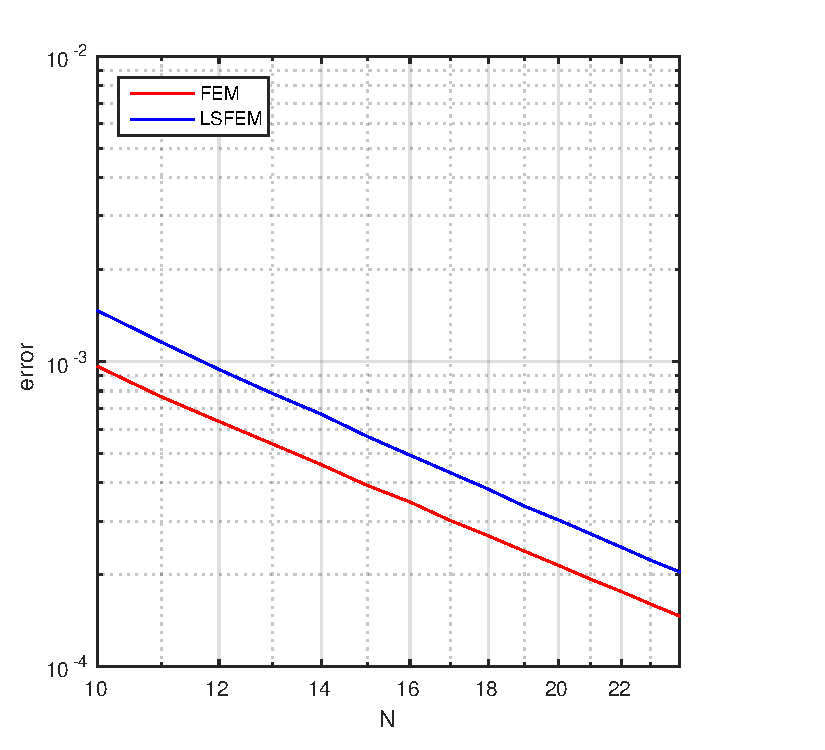
\includegraphics[width=\textwidth]{Figures/errorFEM-LSFEM.pdf}
  \end{subfigure}%
  \quad
  \begin{subfigure}[b]{0.48\textwidth}
	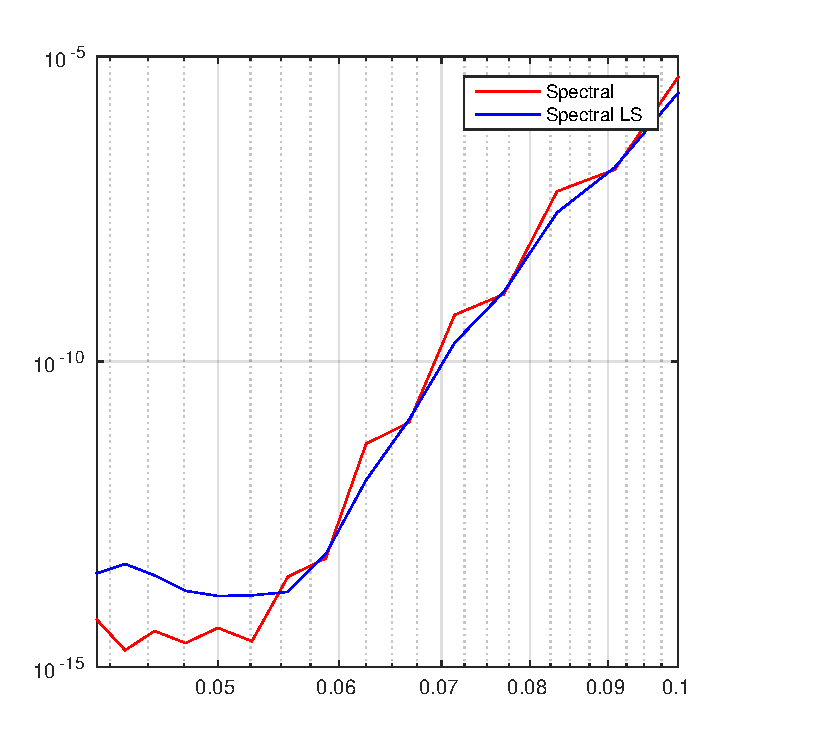
\includegraphics[width=\textwidth]{Figures/errorSpec-SpecLS.pdf}
  \end{subfigure}
          %(or a blank line to force the subfigure onto a new line)
  \vspace{-0.1\baselineskip}
  \caption{Convergence of Galerkin and corresponding least-squares formulation on the Poisson problem.}
  \label{fig:ConvergencePoisson}
\end{figure}
%
\begin{figure}[h!]
  \centering
  \begin{subfigure}[b]{0.48\textwidth}
	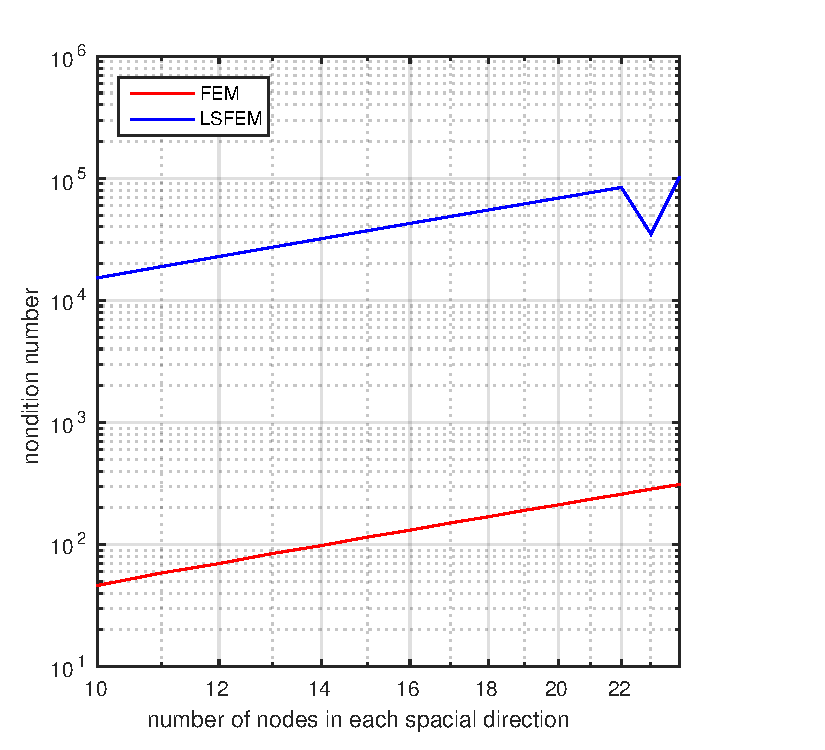
\includegraphics[width=\textwidth]{Figures/condFEM-LSFEM.pdf}
  \end{subfigure}%
  \quad
  \begin{subfigure}[b]{0.48\textwidth}
	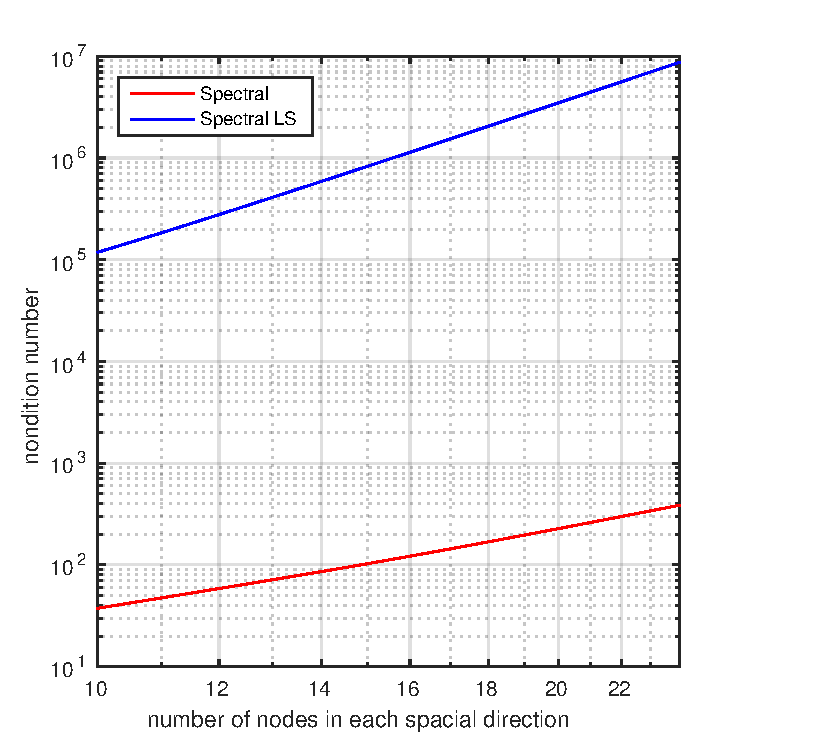
\includegraphics[width=\textwidth]{Figures/condSpec-SpecLS.pdf}
  \end{subfigure}
          %(or a blank line to force the subfigure onto a new line)
  \vspace{-0.1\baselineskip}
  \caption{Condition number of Galerkin and corresponding least-squares formulation on the Poisson problem.}
  \label{fig:ConditionPoisson}
\end{figure}

%\begin{figure}[hl]
	%\centering
  %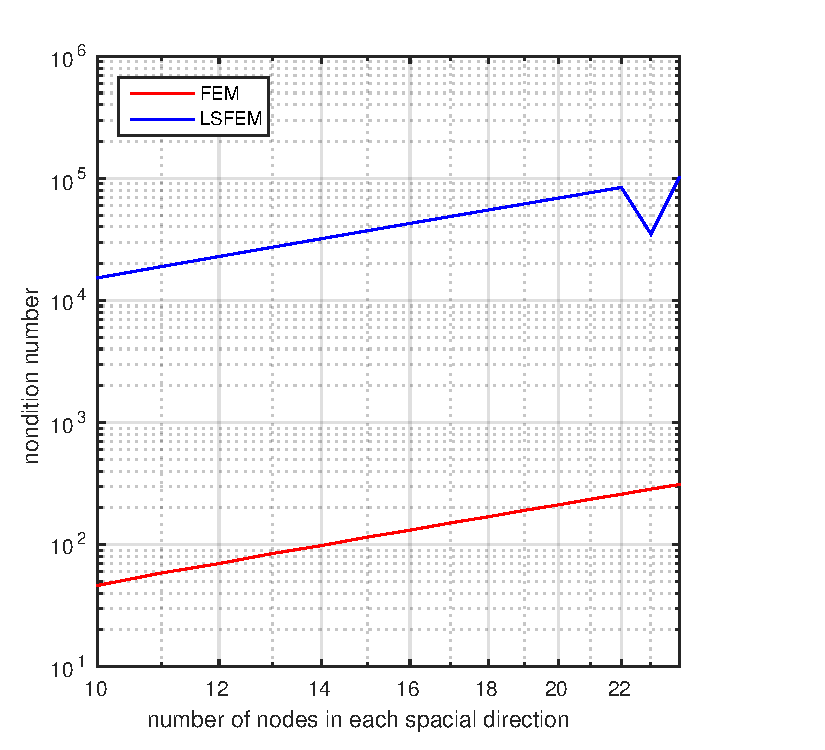
\includegraphics[width=80mm]{Figures/condFEM-LSFEM.pdf}
	%\caption{condition number of LSFEM and FEM}
	%\label{fig:conditionFEM}
%\end{figure}
%%
%%
%\begin{figure}[hl]
	%\centering
	%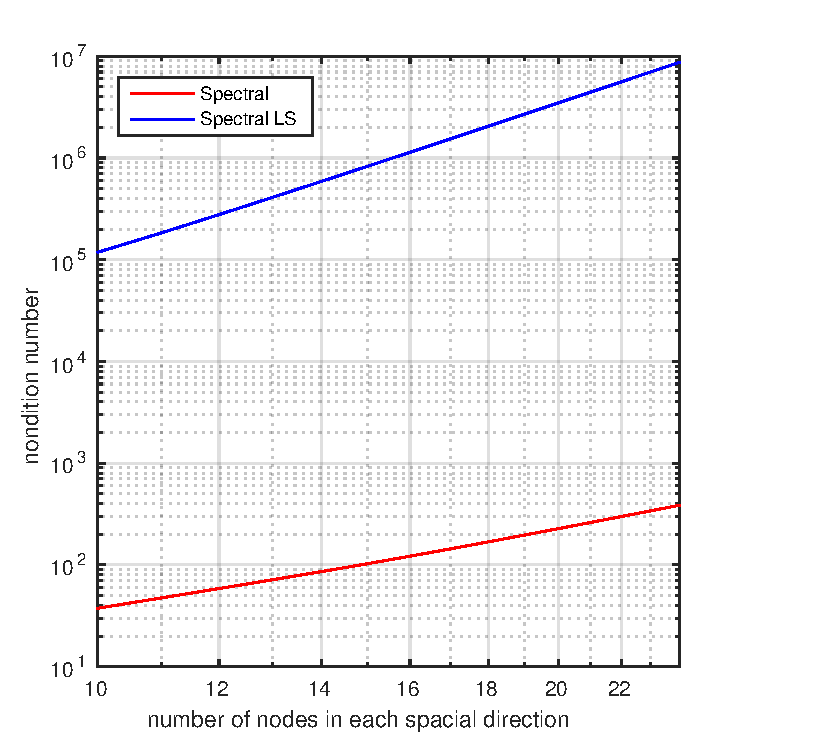
\includegraphics[width=80mm]{Figures/condSpec-SpecLS.pdf}
	%\caption{condition number of Spectral and LS-Spectral method}
	%\label{fig:conditionSpec}
%\end{figure}
%%

 
%\input{Chapters/Chapter5} 
%\input{Chapters/Chapter6} 
%\input{Chapters/Chapter7} 

%----------------------------------------------------------------------------------------
%	THESIS CONTENT - APPENDICES
%----------------------------------------------------------------------------------------

\addtocontents{toc}{\vspace{2em}} % Add a gap in the Contents, for aesthetics

\appendix % Cue to tell LaTeX that the following 'chapters' are Appendices

% Include the appendices of the thesis as separate files from the Appendices folder
% Uncomment the lines as you write the Appendices

% Appendix A

\chapter{Appendix Title Here} % Main appendix title

\label{AppendixA} % For referencing this appendix elsewhere, use \ref{AppendixA}

\lhead{Appendix A. \emph{Appendix Title Here}} % This is for the header on each page - perhaps a shortened title

Write your Appendix content here.
%\input{Appendices/AppendixB}
%\input{Appendices/AppendixC}

\addtocontents{toc}{\vspace{2em}} % Add a gap in the Contents, for aesthetics

\backmatter

%----------------------------------------------------------------------------------------
%	BIBLIOGRAPHY
%----------------------------------------------------------------------------------------

\label{Bibliography}

\lhead{\emph{Bibliography}} % Change the page header to say "Bibliography"

\bibliographystyle{unsrtnat} % Use the "unsrtnat" BibTeX style for formatting the Bibliography

\bibliography{Bibliography} % The references (bibliography) information are stored in the file named "Bibliography.bib"

\end{document}  
